\documentclass[a4paper,11pt]{report}
\usepackage[utf8x]{inputenc}
\usepackage{amsmath} % AMS Math Package
\usepackage{amsthm} % Theorem Formatting
\usepackage{amssymb}	% Math symbols such as \mathbb
\usepackage[pdftex]{graphicx} % Allows for eps images
%\usepackage{multicol} % Allows for multiple columns
%\usepackage[dvips,letterpaper,margin=2in,bottom=2in]{geometry}
%\usepackage{geometry}
\usepackage{booktabs}
\usepackage{enumerate}
\usepackage{verbatim}
\usepackage{fancyhdr}
\usepackage{titlesec}
\usepackage{longtable}
\usepackage{subfigure}
\usepackage{hyperref}
\usepackage{float}
\pagestyle{fancy}
\usepackage[italian]{babel}
\usepackage{graphicx}
\usepackage{latexsym}
\usepackage{verbatim} % commenti estesi
\usepackage{geometry}
\geometry{a4paper,top=3cm,bottom=3cm,left=2.5cm,right=2.5cm,%
heightrounded,bindingoffset=5mm}
\fancyhf{}
%\fancyhead[LE,RO]{\slshape \rightmark}
\fancyhead[LO,RE]{\slshape \leftmark}
\fancyfoot[C]{\thepage}
%\titleformat{\chapter}%
%[display]{\vspace{2cm}\Large\bfseries}{\Huge\thechapter \ \hrulefill}{0pt}{\vspace{4mm}}%
%{\Large\bfseries\filcenter}

%%%%%%%%%%%%%%%%%%%%%%%%%%%%%%%%%%%%%%%%%%%%%%%%%%%%%%%%%%%%%%%%%%%%%%%%%%%%%%%%%%%%%%%%%%%%%%%%%%%%%%%%%%%%%%%%%%%%%%%%%%%%%%%%%%%%%%%%
%Mathematical Commands
%%%%%%%%%%%%%%%%%%%%%%%%%%%%%%%%%%%%%%%%%%%%%%%%%%%%%%%%%%%%%%%%%%%%%%%%%%%%%%%%%%%%%%%%%%%%%%%%%%%%%%%%%%%%%%%%%%%%%%%%%%%%%%%%%%%%%%%%%%
 % Sets margins and page size
%\pagestyle{empty} % Removes page numbers
\makeatletter % Need for anything that contains an @ command
% \DeclareMathOperator{\Sample}{Sample}
\let\vaccent=\v % rename builtin command \v{} to \vaccent{}
\renewcommand{\v}[1]{\ensuremath{\mathbf{#1}}} % for vectors
\newcommand{\gv}[1]{\ensuremath{\mbox{\boldmath$ #1 $}}}
% for vectors of Greek letters
\newcommand{\uv}[1]{\ensuremath{\mathbf{\hat{#1}}}} % for unit vector
\newcommand{\abs}[1]{\left| #1 \right|} % for absolute value
\newcommand{\avg}[1]{\left< #1 \right>} % for average
\let\underdot=\d % rename builtin command \d{} to \underdot{}
\renewcommand{\d}[2]{\frac{d #1}{d #2}} % for derivatives
\newcommand{\dd}[2]{\frac{d^2 #1}{d #2^2}} % for double derivatives
\newcommand{\pd}[2]{\frac{\partial #1}{\partial #2}}
% for partial derivatives
\newcommand{\pdd}[2]{\frac{\partial^2 #1}{\partial #2^2}}
% for double partial derivatives
\newcommand{\pdc}[3]{\left( \frac{\partial #1}{\partial #2}
 \right)_{#3}} % for thermodynamic partial derivatives
\newcommand{\ket}[1]{\left| #1 \right>} % for Dirac bras
\newcommand{\bra}[1]{\left< #1 \right|} % for Dirac kets
\newcommand{\braket}[2]{\left< #1 \vphantom{#2} \right|
 \left. #2 \vphantom{#1} \right>} % for Dirac brackets
\newcommand{\matrixel}[3]{\left< #1 \vphantom{#2#3} \right|
 #2 \left| #3 \vphantom{#1#2} \right>} % for Dirac matrix elements
\newcommand{\grad}[1]{\gv{\nabla} #1} % for gradient
\let\divsymb=\div % rename builtin command \div to \divsymb
\renewcommand{\div}[1]{\gv{\nabla} \cdot #1} % for divergence
\newcommand{\curl}[1]{\gv{\nabla} \times #1} % for curl
\let\baraccent=\= % rename builtin command \= to \baraccent
\renewcommand{\=}[1]{\stackrel{#1}{=}} % for putting numbers above =
\newtheorem{prop}{Proposition}
\newtheorem{thm}{Theorem}[section]
\newtheorem{lem}[thm]{Lemma}
\theoremstyle{definition}
\newtheorem{dfn}{Definition}
\theoremstyle{remark}
\newtheorem*{rmk}{Remark}
\newcommand{\p}[2]{ \frac{ \partial #1}{ \partial #2}} %derivata partiale
\newcommand{\lap}{\nabla^2} %laplaciano
\newcommand{\ham}{\mathcal{H}} % Simbolo dell'hamiltoniana
\newcommand{\rint}{\int_\mathbb{R}} % Integrale su R
\newcommand{\modq}[1]{| #1|^2} % Modulo quadro di ``argomento''
\newcommand{\navg}[2]{\left< #1 ^{#2} \right>} %media di ``arg''^n
\newcommand{\con}[1]{\overline{#1}} %coniugato con la barra
\newcommand{\ih}{\frac{i}{\hbar}} % i/h tagliato
\newenvironment{sistem}%
{\left\lbrace\begin{array}{@{}l@{}}}%
{\end{array}\right.}

\newenvironment{myfig}[1][]{%
\begin{center}%
 \begin{figure}[#1]%
  \centering%
  }{%
  \end{figure}%
  \end{center}%
  }




\begin{document}

\newcommand{\HRule}{\rule{\linewidth}{0.5mm}}
\begin{titlepage}
 \begin{center}
  \HRule \\[0.4cm]
{ \huge \bfseries Laboratorio di \\
fisica computazionale}\\[0.4cm]
\HRule \\[1cm]
\begin{flushleft} \Large
Carlo \textsc{Sana} 
\end{flushleft}

\begin{flushright} \Large
	mat. 726409
\end{flushright}
\HRule \\[1cm]
%\begin{flushright}
%\includegraphics[width=0.7\textwidth,]{title.png}
%\end{flushright}

\end{center}

\end{titlepage}



\section{Modello di Ising}
Il modello è stato implementato su un reticolo bidimensione di larghezza N e inizializzando gli spin al valore $\pm 1 $  con uguale probabilità.
Sono stati implementati due algoritmi: Metropolis e Swendsen-Wang.\\

\subsection{Algoritmo Metropolis}
\subsubsection{Termalizzazione}
Possiamo valutare quando avviene la corretta termalizzazione del sistema analizzando l'andamento della magnetizzazione e dell'energia in funzione del tempo markoviano.
Di seguito è riportato l'andamento dell'energia durante la termalizzazione a due diverse temperature, di cui una è la temperatura critica:\\
\begin{figure}[h]
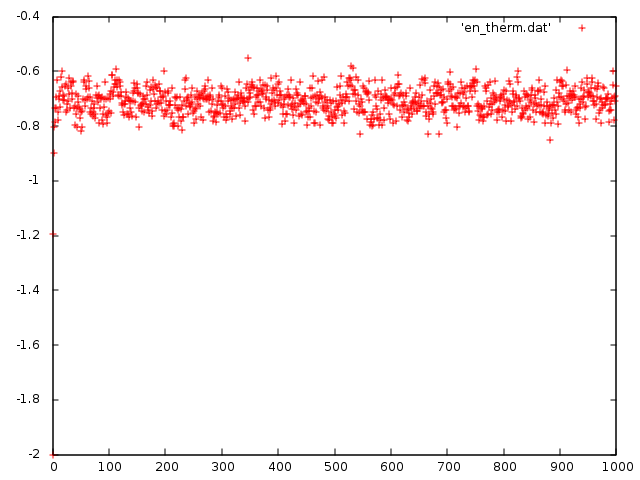
\includegraphics[scale=0.35]{metropolis/en_therm.png}
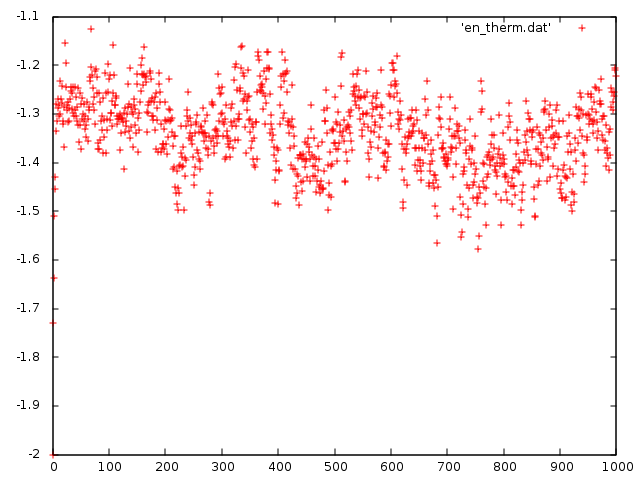
\includegraphics[scale=0.35]{metropolis/en_therm_crit.png}
\caption{Energia a $\beta=0.3$ e $\beta=0.43$}
\end{figure}
\\
Di seguito la magnetizzazione:\\
\begin{figure}[h]
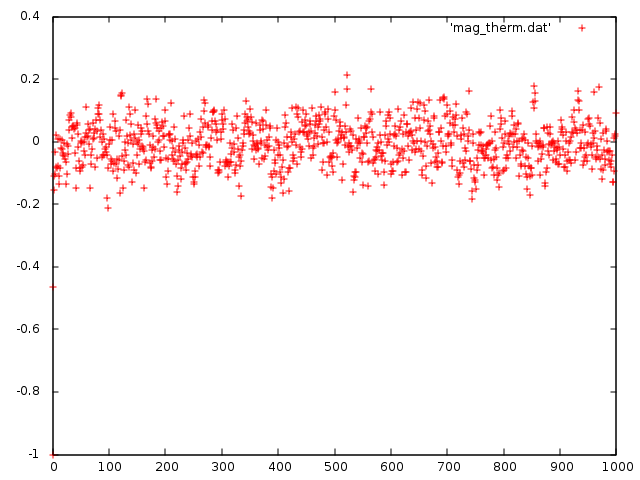
\includegraphics[scale=0.35]{metropolis/mag_therm.png}
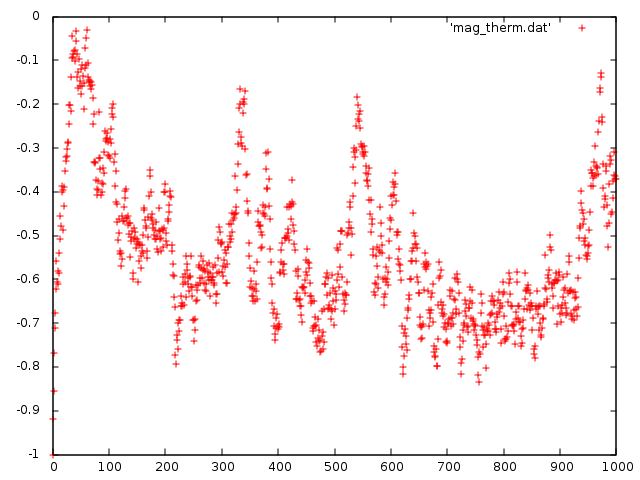
\includegraphics[scale=0.35]{metropolis/mag_therm_crit.png}
\caption{Magnetizzazione a $\beta=0.3$ e $\beta=0.43$}
\end{figure}
Come si può vedere dal grafico relativo alla magnetizzazione a $\beta=0.43$, vicino al punto critico il tempo di termalizzazione cresce di molto. Esso rimane comunque intorno a 100 alla temperatura critica.
Dopo l'analisi di questi dati si è deciso di fissare il tempo di termalizzazione a 1000 passi temporali.

\subsubsection{Autocorrelazione fra le configurazioni}




\end{document}
